%%%%%%%%%%%%%%%%%%%%%%%%%%%%%%%%%%%%%%%%%%%%%%%%%%%%%%%%%%%%%%%%%%%%%%
%%  disstemplate.tex, to be compiled with latex.		     %
%%  08 April 2002	Version 4				     %
%%%%%%%%%%%%%%%%%%%%%%%%%%%%%%%%%%%%%%%%%%%%%%%%%%%%%%%%%%%%%%%%%%%%%%
%%								     %
%%  Writing a Doctoral Dissertation with LaTeX at		     %
%%	the University of Texas at Austin			     %
%%								     %
%%  (Modify this ``template'' for your own dissertation.)	     %
%%								     %
%%%%%%%%%%%%%%%%%%%%%%%%%%%%%%%%%%%%%%%%%%%%%%%%%%%%%%%%%%%%%%%%%%%%%%


\documentclass[12pt]{report}	% The documentclass must be ``report''.

\usepackage{utdiss2}  		% Dissertation package style file.


%%%%%%%%%%%%%%%%%%%%%%%%%%%%%%%%%%%%%%%%%%%%%%%%%%%%%%%%%%%%%%%%%%%%%%
% Optional packages used for this sample dissertation. If you don't  %
% need a capability in your dissertation, feel free to comment out   %
% the package usage command.					     %
%%%%%%%%%%%%%%%%%%%%%%%%%%%%%%%%%%%%%%%%%%%%%%%%%%%%%%%%%%%%%%%%%%%%%%

\usepackage{amsmath,amsthm,amsfonts,amscd, amssymb} 
				% Some packages to write mathematics.
\usepackage{eucal} 	 	% Euler fonts
\usepackage{verbatim}      	% Allows quoting source with commands.
\usepackage{makeidx}       	% Package to make an index.
\usepackage{psfig}         	% Allows inclusion of eps files.
\usepackage{epsfig}         	% Allows inclusion of eps files.
%\usepackage{citesort}         	% 
\usepackage{url}		% Allows good typesetting of web URLs.
%\usepackage{draftcopy}		% Uncomment this line to have the
				% word, "DRAFT," as a background
				% "watermark" on all of the pages of
				% of your draft versions. When ready
				% to generate your final copy, re-comment
				% it out with a percent sign to remove
				% the word draft before you re-run
				% Makediss for the last time.

%The Rest of these are packages that I need for my thesis.
\usepackage{hyperref}
\usepackage{amsfonts}
\usepackage{graphicx}
\usepackage[english]{babel}
%\usepackage[
%backend=biber,
%style=ieee,
%sorting=ynt
%]{biblatex}
\usepackage{tikz}
\usepackage{algorithm}
\usepackage{algorithmicx}
\usepackage[noend]{algpseudocode}
\usepackage{geometry}
\usepackage{marginnote}
\usepackage{csquotes}

%\addbibresource{bibliography.bib}



\author{Matthew Alexander Denend}  	% Required

%Used email address as I STRONGLY preferred this as opposed 
%to physical address. 
\address{mad4672@cs.utexas.edu}  % Required

\title{Challenging Variants of the Collatz Conjecture}
                                                    % Required

%%%%%%%%%%%%%%%%%%%%%%%%%%%%%%%%%%%%%%%%%%%%%%%%%%%%%%%%%%%%%%%%%%%%%%
% NOTICE: The total number of supervisors and other members %%%%%%%%%%
%%%%%%%%%%%%%%% MUST be seven (7) or less! If you put in more, %%%%%%%
%%%%%%%%%%%%%%% they are put on the page after the Committee %%%%%%%%%
%%%%%%%%%%%%%%% Certification of Approved Version page. %%%%%%%%%%%%%%
%%%%%%%%%%%%%%%%%%%%%%%%%%%%%%%%%%%%%%%%%%%%%%%%%%%%%%%%%%%%%%%%%%%%%%

%%%%%%%%%%%%%%%%%%%%%%%%%%%%%%%%%%%%%%%%%%%%%%%%%%%%%%%%%%%%%%%%%%%%%%
%
% Enter names of the supervisor and co-supervisor(s), if any,
% of your dissertation committee. Put one name per line with
% the name in square brackets. The name on the last line, however,
% must be in curly braces.
%
% If you have only one supervisor, the entry below will read:
%
%	\supervisor
%		{Supervisor's Name}
%
% NOTE: Maximum three supervisors. Minimum one supervisor.
% NOTE: The Office of Graduate Studies will accept only two supervisors!
% 
%
\supervisor
	[Scott Aaronson]
	{Marienus Heule}

%%%%%%%%%%%%%%%%%%%%%%%%%%%%%%%%%%%%%%%%%%%%%%%%%%%%%%%%%%%%%%%%%%%%%%
%
% Enter names of the other (non-supervisor) members(s) of your
% dissertation committee. Put one name per line with the name
% in square brackets. The name on the last line, however, must
% be in curly braces.
%
% NOTE: Maximum six other members. Minimum zero other members.
% NOTE: The Office of Graduate Studies may restrict you to a total
%	of six committee members.
%
%
%\committeemembers
%	[Erwin Schr\"odinger]
%	[Albert Einstein]
%	[Charles Townes]
%	{Arthur Schawlow}

%%%%%%%%%%%%%%%%%%%%%%%%%%%%%%%%%%%%%%%%%%%%%%%%%%%%%%%%%%%%%%%%%%%%%%

\previousdegrees{B.S.}
     % The abbreviated form of your previous degree(s).
     % E.g., \previousdegrees{B.S., MBA}.
     %
     % The default value is `B.S., M.S.'

%\graduationmonth{...}      
     % Graduation month, either May, August, or December, in the form
     % as `\graduationmonth{May}'. Do not abbreviate.
     %
     % The default value (either May, August, or December) is guessed
     % according to the time of running LaTeX.

%\graduationyear{...}   
     % Graduation year, in the form as `\graduationyear{2001}'.
     % Use a 4 digit (not a 2 digit) number.
     %
     % The default value is guessed according to the time of 
     % running LaTeX.

%\typist{...}       
     % The name(s) of typist(s), put `the author' if you do it yourself.
     % E.g., `\typist{Maryann Hersey and the author}'.
     %
     % The default value is `the author'.


%%%%%%%%%%%%%%%%%%%%%%%%%%%%%%%%%%%%%%%%%%%%%%%%%%%%%%%%%%%%%%%%%%%%%%
% Commands for master's theses and reports.			     %
%%%%%%%%%%%%%%%%%%%%%%%%%%%%%%%%%%%%%%%%%%%%%%%%%%%%%%%%%%%%%%%%%%%%%%
%
% If the degree you're seeking is NOT Doctor of Philosophy, uncomment
% (remove the % in front of) the following two command lines (the ones
% that have the \ as their second character).
%
\degree{MASTER OF SCIENCE IN COMPUTER SCIENCE}
\degreeabbr{M.S. Comp.Sci.}

% Uncomment the line below that corresponds to the type of master's
% document you are writing.
%
%\masterreport
\masterthesis


%%%%%%%%%%%%%%%%%%%%%%%%%%%%%%%%%%%%%%%%%%%%%%%%%%%%%%%%%%%%%%%%%%%%%%
% Some optional commands to change the document's defaults.	     %
%%%%%%%%%%%%%%%%%%%%%%%%%%%%%%%%%%%%%%%%%%%%%%%%%%%%%%%%%%%%%%%%%%%%%%
%
%\singlespacing
%\oneandonehalfspacing

%\singlespacequote
\oneandonehalfspacequote

\topmargin 0.125in	% Adjust this value if the PostScript file output
			% of your dissertation has incorrect top and 
			% bottom margins. Print a copy of at least one
			% full page of your dissertation (not the first
			% page of a chapter) and measure the top and
			% bottom margins with a ruler. You must have
			% a top margin of 1.5" and a bottom margin of
			% at least 1.25". The page numbers must be at
			% least 1.00" from the bottom of the page.
			% If the margins are not correct, adjust this
			% value accordingly and re-compile and print again.
			%
			% The default value is 0.125"

		% If you want to adjust other margins, they are in the
		% utdiss2-nn.sty file near the top. If you are using
		% the shell script Makediss on a Unix/Linux system, make
		% your changes in the utdiss2-nn.sty file instead of
		% utdiss2.sty because Makediss will overwrite any changes
		% made to utdiss2.sty.

%%%%%%%%%%%%%%%%%%%%%%%%%%%%%%%%%%%%%%%%%%%%%%%%%%%%%%%%%%%%%%%%%%%%%%
% Some optional commands to be tested.				     %
%%%%%%%%%%%%%%%%%%%%%%%%%%%%%%%%%%%%%%%%%%%%%%%%%%%%%%%%%%%%%%%%%%%%%%

% If there are 10 or more sections, 10 or more subsections for a section,
% etc., you need to make an adjustment to the Table of Contents with the
% command \longtocentry.
%
%\longtocentry 



%%%%%%%%%%%%%%%%%%%%%%%%%%%%%%%%%%%%%%%%%%%%%%%%%%%%%%%%%%%%%%%%%%%%%%
%	Some math support.					     %
%%%%%%%%%%%%%%%%%%%%%%%%%%%%%%%%%%%%%%%%%%%%%%%%%%%%%%%%%%%%%%%%%%%%%%
%I USED MY OWN HERE.
%
%	Theorem environments (these need the amsthm package)
%
%% \theoremstyle{plain} %% This is the default
\newtheorem{theorem}{Theorem}[section]
\newtheorem{corollary}{Corollary}[theorem]
\newtheorem{lemma}[theorem]{Lemma}

%\theoremstyle{definition}
%\newtheorem{definition}{Definition}[section]
%\newtheorem{question}{Question}[section]

\newcommand{\Mod}[1]{\ (\mathrm{mod}\ #1)}
\newcommand{\Col}[1]{\mathrm{Col}(#1)}
\newcommand{\ColMod}[3]{\mathrm{Col}_{\text{mod}}(#1,#2,#3)}
%\newtheorem{thm}{Theorem}[section]
%\newtheorem{cor}[thm]{Corollary}
%\newtheorem{lem}[thm]{Lemma}
%\newtheorem{prop}[thm]{Proposition}
%\newtheorem{ax}{Axiom}

%\theoremstyle{definition}
%\newtheorem{defn}{Definition}[section]

%\theoremstyle{remark}
%\newtheorem{rem}{Remark}[section]
%\newtheorem*{notation}{Notation}

%\numberwithin{equation}{section}


%%%%%%%%%%%%%%%%%%%%%%%%%%%%%%%%%%%%%%%%%%%%%%%%%%%%%%%%%%%%%%%%%%%%%%
%	Macros.							     %
%%%%%%%%%%%%%%%%%%%%%%%%%%%%%%%%%%%%%%%%%%%%%%%%%%%%%%%%%%%%%%%%%%%%%%
%
%	Here some macros that are needed in this document:


\newcommand{\latexe}{{\LaTeX\kern.125em2%
                      \lower.5ex\hbox{$\varepsilon$}}}

\newcommand{\amslatex}{\AmS-\LaTeX{}}

\chardef\bslash=`\\	% \bslash makes a backslash (in tt fonts)
			%	p. 424, TeXbook

\newcommand{\cn}[1]{\texttt{\bslash #1}}

\makeatletter		% Starts section where @ is considered a letter
			% and thus may be used in commands.
\def\square{\RIfM@\bgroup\else$\bgroup\aftergroup$\fi
  \vcenter{\hrule\hbox{\vrule\@height.6em\kern.6em\vrule}%
                                              \hrule}\egroup}
\makeatother		% Ends sections where @ is considered a letter.
			% Now @ cannot be used in commands.

\makeindex    % Make the index

%%%%%%%%%%%%%%%%%%%%%%%%%%%%%%%%%%%%%%%%%%%%%%%%%%%%%%%%%%%%%%%%%%%%%%
%		The document starts here.			     %
%%%%%%%%%%%%%%%%%%%%%%%%%%%%%%%%%%%%%%%%%%%%%%%%%%%%%%%%%%%%%%%%%%%%%%

\begin{document}

\copyrightpage          % Produces the copyright page.


%
% NOTE: In a doctoral dissertation, the Committee Certification page
%		(with signatures) is BEFORE the Title page.
%	In a masters thesis or report, the Signature page
%		(with signatures) is AFTER the Title page.
%
%	If you are writing a masters thesis or report, you MUST REVERSE
%	the order of the \commcertpage and \titlepage commands below.
%
\commcertpage           % Produces the Committee Certification
			%   of Approved Version page (doctoral)
			%   or Signature page (masters).
			%		20 Mar 2002	cwm

\titlepage              % Produces the title page.



%%%%%%%%%%%%%%%%%%%%%%%%%%%%%%%%%%%%%%%%%%%%%%%%%%%%%%%%%%%%%%%%%%%%%%
% Dedication and/or epigraph are optional, but must occur here.      %
%%%%%%%%%%%%%%%%%%%%%%%%%%%%%%%%%%%%%%%%%%%%%%%%%%%%%%%%%%%%%%%%%%%%%%
%
\begin{dedication}
\index{Dedication@\emph{Dedication}}%
Dedicated to my late mother, who passed away earlier this year, yet never
let her three battles with cancer stop her from endlessly loving her sons and
her husband.
\end{dedication}


\begin{acknowledgments}		% Optional
\index{Acknowledgments@\emph{Acknowledgments}}%
I want to give a huge thank you to both of my advisors for this project: Scott Aaronson and Marijn Heule. \par
Scott Aaronson came to UT Austin from MIT in fall 2016. I knew that I wanted to write a Master's Thesis from pretty much the time I started my Master's Degree, and I heard he might be a great person to work with. We come from very different backgrounds. He is well-renowned for his work in Theoretical Quantum Computing. I came into UT's CS program with virtually no Math/CS theory background, as my undergrad degree was in Electrical Engineering. At one point, he suggested that I talk to Marijn Heule, and hence, this project was born. I got a chance to witness firsthand the enthusiasm that Scott has for CS and Math theory, and it's no wonder that Scott has done so much work in Theoretical Computer Science... he just keeps going and going! This entire project would not have been possible without him and he is as much, if not more, of an author of this Thesis as I am. I'm also deeply thankful to him for his support as I had to go through the challenge of losing my mom.\par
Marijn Heule became an Assistant Research Professor at UT in fall 2017. He was a Research Scientist at UT Austin when I first met him. Marijn is a master at SAT Solving, and is famous for his proof of the Boolean Pythagorean Triples problem that was the largest proof ever at the time at 100 TB. Much like Scott, Marijn has a great deal of enthusiasm for mathematical problems. This entire project is originally Marijn's idea, so I am thankful that he had this idea, and I am very happy to have written a Thesis with such a cool topic. Without his advice and direction and his many read-overs and edits, this Thesis would have not been possible to finish, so he is as much, if not more, of an author of this Thesis as I am. I am also deeply thankful of the support he gave me as I had to go through the challenge of losing my mom.\par
When Scott and Marijn first met each other, they raced each other to solve several proofs related to this project: Scott by hand, Marijn using computation. I happened to be in the middle of it all, unable to keep up with the blazing speed of these two brilliant minds. It took me some time but I can now confidently read through these original thoughts that Scott and Marijn had and understand most of them much better now then when they first occurred. \par
I am forever indebted to these two men and can only hope to someday achieve the greatness and brilliance of them. \par
I am also thankful for the many friends that I have made along the way towards finishing this Thesis, especially those who gave me support as I had to deal with the loss of my mom. There are far too many to list, but you know who you are. From my time here in Austin, I have made many friends that I want to keep for many years to come.
\end{acknowledgments}


% The abstract is required. Note the use of ``utabstract'' instead of
% ``abstract''! This was necessary to fix a page numbering problem.
% The abstract heading is generated automatically.
% Do NOT use \begin{abstract} ... \end{abstract}.
%
\utabstract
\index{Abstract}%
\indent
%Should not exceed 350 words. Looks like I have a good amount.
The Collatz Conjecture (also known as the $3x+1$ problem) is simple to explain, yet proving that all positive integers following the Collatz map must converge to 1 has eluded mathematicians for over half a century. Aaronson and Heule are exploring solving the Collatz Conjecture using an approach involving string rewrite systems: Aaronson transformed the Conjecture into a string rewrite system and Heule applied parallel SAT solvers on instances of this system. Similar approaches have been applied successfully to other mathematical problems.\par
We started looking into simpler, but also challenging variants of the conjecture. This thesis defines some of these variants and investigates easily provable as well as very hard variants. We study the hardness of unsolved variants by computing the number of rewrite steps needed up to 1 billion. Our hardness prediction method suggests that proving termination of the challenging variants should be considerably easier compared to solving the original conjecture.
\tableofcontents   % Table of Contents will be automatically
                   % generated and placed here.

%\listoftables      % List of Tables and List of Figures will be placed
\listoffigures     % here, if applicable.



%%%%%%%%%%%%%%%%%%%%%%%%%%%%%%%%%%%%%%%%%%%%%%%%%%%%%%%%%%%%%%%%%%%%%%
% Actual text starts here.					     %
%%%%%%%%%%%%%%%%%%%%%%%%%%%%%%%%%%%%%%%%%%%%%%%%%%%%%%%%%%%%%%%%%%%%%%
%
% Including external files for each chapter makes this document simpler,
% makes each chapter simpler, and allows for generating test documents
% with as few as zero chapters (by commenting out the include statements).
% This allows quicker processing by the Makediss command file in case you
% are not working on a specific, long and slow to compile chapter. You
% can even change the chapter order by merely interchanging the order
% of the include statements (something I found helpful in my own
% dissertation).
%
\chapter{Introduction} \label{sec:introduction}
Computers have been successfully applied to many complex problems, such as those in finance, healthcare, and the Internet. However, computers still struggle with several problems. Consider whether a given program on any input will always terminate. One can easily show that certain programs will always halt. For example, we can easily show a program that takes an integer input $x$, computes $y=x+1$, prints $y$, then halts, will always terminate. Nevertheless, there exist simple programs that are much harder to determine if they always terminate. Algorithm~\ref{alg:ColR} is such an example. Will this program always return 1 for any positive integer $N$, causing it to halt? This problem is a reformulation of the Collatz Conjecture, also known as the $3N+1$ problem. \par
\begin{algorithm} 
\caption{The Collatz Conjecture Sequence, $\Col{N}$}
\label{alg:ColR} 
\begin{algorithmic}[1]
    \If{$N \leq 1$} \Return $N$ 
    \EndIf
    \If {$N \equiv 0 \Mod{2}$} \Return $\Col{N/2}$
    \EndIf
    \State \Return $\Col{3N + 1}$ 
\end{algorithmic}
\end{algorithm}
We know from Turing that no program exists to determine if an arbitrary program with arbitrary input can halt~\cite{Turing1936}, but that does not exclude the possibility of a program that determines if specifically Algorithm~\ref{alg:ColR} halts. However, no program has been found to show that all positive integer inputs for Algorithm~\ref{alg:ColR} will halt, even though this problem can be explained to an elementary grade student. The problem has been extensively analyzed, according to surveys by Lagrias~\cite{2003mathLagrais}~\cite{2006mathLagrias}, yet no proof has been found. The search is further motivated by extensive empirical evidence suggesting that the Collatz Conjecture is true. According to a website maintained by Roosendahl~\cite{EricRoose}, all numbers up to $87 \cdot 2^{60}$, or about $10^{20}$, have been tried as $N$ in Algorithm~\ref{alg:ColR}, and have converged to 1. \par
Since the Collatz Conjecture has been challenging to prove, we propose another supposedly simpler variant of it. Can we prove that the code in Algorithm \ref{alg:ColSP}, where $A = \{1\}$, and $b = 8$, always terminates for any positive integer $N$? Even though this program seems to be easier, we do not have a program showing this variant always terminates either! \par
\begin{algorithm} 
\caption{A Collatz Conjecture Variant $\ColMod{N}{A}{b}$}
\label{alg:ColSP} 
\begin{algorithmic}[1]
    \If{$(N \leq 1) \vee (N \equiv a_1  \Mod{b}) \vee \ldots \vee (N \equiv a_s \Mod{b})$ } \Return $N$
    \EndIf
    \If {$N \equiv 0 \Mod{2}$} \Return $\ColMod{N/2}{A}{b}$
    \EndIf
    \State \Return $\ColMod{3N+1}{A}{b}$ 
\end{algorithmic}
\end{algorithm}
One of the goals of this thesis is to try and determine how hard certain variants of the Collatz Conjecture are to solve. A contribution of this thesis is that it uses empirical data to try and find trends of hardness for difficult variants, and compare these trends to the hardness of solving the whole Collatz Conjecture. This thesis also follows an approach that Heule and Aaronson have devised attempting to craft a program to determine if Algorithm~\ref{alg:ColR} always halts~\cite{HeuleAaronson}. At a high level, it involves taking a completely reworked formulation of Algorithm~\ref{alg:ColR} and using known techniques that, if certain conditions are met, the reworked formulation can be shown to terminate for any positive integer input. The formulation requires SAT solvers, string rewrite systems, and a technique called matrix interpretation, all topics which will be covered briefly in this paper as background. This thesis also investigates a rewrite system that Aaronson crafted, and we believe that, if Aaronson's system is found to terminate for all input, the Collatz Conjecture holds. We analyze properties of this rewrite system, and the previously variants are investigated with this rewrite system as well.\par
The rest of this thesis is outlined as follows: Chapter~\ref{sec:defns} introduces definitions that will be used throughout the paper. Chapter~\ref{sec:alttercdns} defines several Collatz Conjecture Variants, both solved and unsolved, including $\ColMod{N}{\{1\}}{8})$. Chapter~\ref{sec:subhrdnspred} analyzes the difficulty of these variants using algebra. Chapter ~\ref{sec:SRSandSAT} discusses the results so far of Heule using Aaronson's rewrite system and parallel SAT solving to prove the Collatz Conjecture and hard Collatz Variants, as well as necessary background to understand the approach. Finally, Chapter~\ref{sec:hardnessrewriterules} investigates hardness of solving the same variants covered in Chapter~\ref{sec:subhrdnspred}, but derived from Aaronson's rewrite system instead.
%%  LocalWords:  healthcare Lagrias


\chapter{Definitions} \label{sec:defns}
We will use the following terms throughout this Thesis:
\begin{itemize}
    \item $\boldsymbol{3x+1}$\textbf{ mapping}: A one step application of $\Col{N}$ to some input number $N$.
    \item $\boldsymbol{3x+1}$\textbf{ sequence}: Define this as follows: 
    \begin{align*}
        x_0 = x &= \text{ initial input number} \\
        x_{i+1} &= \begin{cases} 
        x_{i}/2 &\text{ if $x_i$ is even} \\
        3 x_{i} + 1 &\text{ if $x_i$ is odd} \\
        \end{cases}
    \end{align*}
    This sequence can continue for arbitrarily large values of $i$, but we are only interested in following the sequence until $x_i$, for some $i$, is 1, as any value after 1 follows the cycle of $1 \rightarrow 4 \rightarrow 2 \rightarrow 1$ infinitely.
    \item \textbf{Avoidance set $\boldsymbol A$:} The second parameter of Algorithm~\ref{alg:ColSP}, which was defined in the introduction. $A = \{a_1 \ldots a_s\}$ is all of the numbers modulo the positive integer $b$ (the third parameter of Algorithm~\ref{alg:ColSP}) that cause termination of the algorithm. This termination condition is in addition to the sole termination condition of Algorithm~\ref{alg:ColR}: when the input number $N$ is 1. Note that for all $a \in A$, $0 \le a < b$, and $A = \varnothing$ turns Algorithm~\ref{alg:ColSP} into Algorithm~\ref{alg:ColR}.
    \item \textbf{Collatz Variant:} When we say ``Collatz Variant'' we are referring to Algorithm~\ref{alg:ColSP}, for some positive integer $N$, avoidance set $A$, and positive integer $b$. There are a couple of shorthands we use throughout this Thesis:
      \begin{itemize}
      \item $\boldsymbol{\ColMod{N}{A}{b}:}$ Parameters are the same as Algorithm~\ref{alg:ColSP}.
      \item \textbf{Collatz Variant A:} The vast majority of our analysis is when $b = 8$, so when we say Collatz Variant $A$, it is shorthand for $\ColMod{N}{A}{8}$. For singleton sets $A$, we omit the braces normally around sets. We often list several Collatz Variants together, so for instance, if we say Collatz Variants 1, 5, 7, and $\{1,5\}$, we mean the variants $\ColMod{N}{\{1\}}{8}$, $\ColMod{N}{\{5\}}{8}$, $\ColMod{N}{\{7\}}{8}$, and $\ColMod{N}{\{1,5\}}{8}$, respectively.
      \end{itemize}
\item \textbf{Collatz String Rewrite System (SRS):} Created by Aaronson~\cite{HeuleAaronson}, and introduced in chapter~\ref{sec:SRSandSAT}, along with background on string rewrite systems, this is used in the latter portion of this paper as an alternative way of expressing the Collatz Conjecture. Also called Aaronson's SRS.
\item \textbf{Number of bits:} For an input number $x$, we say that, written in binary, it has $m$ bits.
\end{itemize}
We also have definitions within Chapter~\ref{sec:subhrdnspred} and~\ref{sec:hardnessrewriterules}. See sections~\ref{subsec:algdefinemeasure} and~\ref{subsec:rewritemeasuredefs}, respectively.
%INSTEAD OF DEFINING SEVERAL THINGS HERE, LET'S DO THE FOLLOWING INSTEAD: Say that these terms will also be used throughout the paper, but will be defined more formally in (give section number)
%Collatz base b Graph
%"Node a:"
%


\chapter{Alternative Termination Conditions} \label{sec:alttercdns}
 This section explores the problem originally presented in Algorithm~\ref{alg:ColM} and defines several other problems related to it. Before we investigate these open variants, we define a graph paradigm that transforms the $3x+1$ problem into directed graphs that depict the flow for all input numbers modulo base $b$, where $b$ is a power of 2. Then using this graph, we can show that some variants are provable, whereas others are not.
 %Instead of trying to directly analyze strings from the rewrite system, we can just compute $3x+1$ sequences directly, and convert numbers back and forth to binary, as needed. Using numbers instead of rewrite strings is far less expensive computationally. Furthermore, if we focus our investigation on the least significant bits of these input numbers, we can easily tie the $D$ rewriting rules, or some modifications thereof, to a graph, which allows us to investigate things such as how many times a rewrite rule can be applied before it cannot be applied anymore, but at a far cheaper cost. We can also analyze the necessity for the odd nodes/rules because odd numbers make the Collatz Conjecture harder to solve, since it causes a number to grow. \par
\section{Defining a Collatz base \textit{b} graph} \label{subsec:colgraph}
Define $G_b=(V,E)$ to be a ``Collatz base $b$ graph'', where $b = 2^k$, and $k$ is nonnegative. Choosing a power of 2 for $b$ allows us to easily reason with binary numbers, which is useful for both several proofs in this section and the String Rewrite System that we will discuss starting in section~\ref{sec:CollatzSRS}. $V$ has $b$ vertices in it, where each vertex is labeled a unique integer in the interval $[0, b-1]$. Vertex $v \in V$ corresponds to $v \Mod{b}$. This paper uses the term ``node $v$'' as shorthand to correspond to the number $v$ in $v \Mod{b}$, as opposed to ``vertex'' $v$ which corresponds to the actual vertex of the graph. Let $x_i$ be the $i$\textsuperscript{th} step of the $3x+1$ sequence for input number $x$, and $x_{i+1}$ be the step after. $E = V \times V$ is a set of directed edges, where, for nodes $u, v \in V$, $(u,v) \in E$ if and only if $x_i \equiv u \Mod{b}$ and $x_{i+1} \equiv v \Mod{b}$ for some $x_i$ and $x_{i+1}$. \par

\section{Lemmas that hold for any base \textit{b} Collatz Graph}
This section contains some lemmas that are used throughout this Thesis. First, we start with a lemma about the number of node transitions in any Collatz base $b$ graph $G_b= (V,E)$.
\begin{lemma}
\label{lem:numOutEdges}
Given a Collatz base $b$ graph, for all $v \in V$, if node $v$ is even, then the vertex $v$ has two outgoing edges. Otherwise, if node $v$ is odd, then the vertex $v$ has only one outgoing edge.
\end{lemma}
\begin{proof}
Take a number $x_i$ that corresponds to node $v$. First, let us consider the case where node $v$ is even. When we divide by 2, we just remove the lowest 0. The new bit at index $k-1$ can be either a 0 or a 1, allowing for two options for even nodes. \par
Now, take $x_i$ that corresponds to a node $v$ that is odd. Multiplying $x_i$ by 3 and adding 1 will make the binary string grow at least one bit longer (since $3\cdot x_i = 2 \cdot x_i + x_i$), giving us only one option for the least significant $k$ bits, meaning $x_{i+1}$ can only correspond to one node $w \in V$, and only one such outgoing edge from $v$ exists.
\end{proof}
Now, we have a couple of important properties about cycles that exist in any Collatz base $b$ graph, and the fact that these cycles cannot continue indefinitely. First, we introduce the ``0 cycle'' Lemma.
\begin{lemma}
\label{lem:zeroCycle}
For any Collatz base $b$ graph (where $b$ is a positive power of 2), a self-loop occurs on a 0 node. This cycle cannot continue indefinitely.
\end{lemma}
\begin{proof}
Assume we have an input number $N$ such that $N \equiv 0 \Mod{b}$. This means that the $k$ least significant bits are all 0. Apply the $3x+1$ mapping once to this string. We remove a 0 from the end, since we divide the input number by 2. We now look at the new number $N/2$ and the $k$ least significant bits. The $k-1$ least significant bits are all 0. But what is the value of the bit in the most significant of the $k$ bits? If it is a 0, then our new number $N/2 \equiv 0 \Mod{b}$, and we have a self-loop. \par
To show that the self loop cannot continue indefinitely: every time we follow the self-loop, remove a 0. Since we also know that $N > 1$ in order for the algorithm to continue running, we also know that at least one binary digit is a 1. So as we continue cutting off 0's, we eventually reach a point where the least $k$ significant bits are $1000\ldots 0$, meaning we transition to node $b/2$ instead, ending the cycle.
\end{proof}
Now, we introduce another important lemma about cycles: the fact that we will always have a cycle between nodes $b-2$ and $b-1$. We call this the ``1 Consumption'' Lemma.
\begin{lemma}
\label{lem:oneConsumption}
 For any Collatz base $b$ graph, a cycle between exists between nodes $b-2$ and $b-1$. This cycle cannot continue indefinitely.
\end{lemma}
\begin{proof}
In this proof, we will show first that a $b-1 \rightarrow b-2 \rightarrow b-1$ cycle exists, and second, that this cycle cannot continue indefinitely; more precisely, that some number congruent modulo to $b-2 \Mod{b}$, after division by 2, actually becomes $b/2-1 \Mod{b}$ instead. We will do so using long multiplication in binary, adding the 1 in as well for shorthand. \par
Let $x$ be a arbitrary number congruent modulo to $b-1 \Mod{b}$. We want to express $x$ in binary, so let $x$ have $m$ bits. We know that since $x$ is congruent modulo to $b-1 \Mod{b}$, all bits from indices 0 to $k-1$ are 1. Let $x_j$ denote the $j$\textsuperscript{th} bit of $x$, $k \leq j \leq m$. These indices correspond to unknown bits. Let $1_{+1}$ correspond to the adding of 1 after multiplying by 3, which is added to the 0\textsuperscript{th} index of $x$. Let $c_j$ denote the unknown carry for the $j$\textsuperscript{th} index of bits being added. Let $y$ be the result after $3x+1$ is computed, and let the $j$\textsuperscript{th} index of $y$ be the same index as $x$. The multiplication is referenced in Table~\ref{tab:mul}. \par
\begin{figure}
\begin{tabular}{*{16}c}%{c*{15}{@{\,}c}}
 & & $ x_{n}$  & $ x_{n-1}$  & \ldots & $ x_{j+1}$  & $ x_{j}$  & \ldots & $ x_{k+1}$  & $ x_{k}$  & 1 & 1 & \ldots & 1 & 1 & 1 \\
$\times$ & & & & & & & & & & & & & & 1 & 1 \\
\hline
\tiny ${\scriptscriptstyle c_{n+2}}$ & ${\scriptscriptstyle c_{n+1}}$ & ${\scriptscriptstyle c_{n}}$ & ${\scriptscriptstyle c_{n-1}}$ & & ${\scriptscriptstyle c_{j+1}}$ & ${\scriptscriptstyle c_{j}}$ & & ${\scriptscriptstyle c_{k+1}}$ & \tiny 1 & \tiny 1 &  \tiny 1 & &  \tiny 1 & \tiny 1 & \\
  & & $ x_{n}$  & $ x_{n-1}$  & \ldots & $ x_{j+1}$  & $ x_{j}$  & \ldots & $ x_{k+1}$  & $ x_{k}$  & 1 & 1 & \ldots & 1 & 1 & 1 \\
  + & $ x_{n}$  & $ x_{n-1}$  & $ x_{n-2}$  & \ldots & $ x_{j}$  & $ x_{j-1}$  & \ldots & $ x_{k}$  & 1 & 1 & 1 & \ldots & 1 & 1 & $1_{+1}$  \\
  \hline
  $ y_{n+2}$  & $ y_{n+1}$  & $ y_{n}$  & $ y_{n-1}$  & \ldots & $ y_{j+1}$  & $ y_{j}$  & \ldots & $ y_{k+1}$  & $ y_{k}$  & 1 & 1 & \ldots & 1 & 1 & 0 
\end{tabular}
\caption{The long multiplication corresponding to $3x + 1$. Note how, in the addition step, the $1_{+1}$ is in place of a zero, and the addition is just $x + 2x + 1$.}
\label{fig:mul}
\end{figure}
Observe that, in binary, multiplication of a binary number $x$ by 3 is just $x + 2x$, and $2x$ is just placing all bits of $x$ one index to the left. In the multiplication we show in Figure~\ref{fig:mul}, we replace the extra 0 vacated by $2x$ with the addition of 1, $1_+1$, allowing us to perform $3x+1$ with just one addition instead of two. \par
Observe that all bits in the resulting binary number $y$ from indices 0 to $k-1$ are 1, except for index 0, which is 0. This is because all bits of $y$, save index 0, are computed by adding $1+1$ and carrying over the 1 from the previous addition. As a result, $y$ is congruent modulo to $b-2 \Mod{b}$, meaning an edge from node $b-1 \Mod{b}$ to node $b-2 \Mod{b}$ exists in our graph.\par
When we divide $y$ by 2, we just remove the lowest 0 from $y$. Hence, bit $y_k$ is now in position $k-1$. If $y_k$ is 1, our number is now congruent modulo to $b-1 \Mod{b}$. This means an edge also exists from node $b-2 \Mod{b}$ to node $b-1 \Mod{b}$, proving the existence of the cycle. \par
Now we show that this $b-2 \rightarrow b-1 \rightarrow b-2$ cycle will always eventually terminate. This happens when, after dividing a number congruent modulo to $b-2 \Mod{b}$ by 2, bit $y_{k-1}$ is 0. So we need to show this eventually occurs for any arbitrary $x$. There are two cases for this:
\begin{enumerate}
    \item Some bit in $x$ is 0. Let $x_j$ be the least significant bit of $x$ that is 0 (all bits which have indices lower than $j$ are 1). Look back at Figure~\ref{fig:mul}, and replace $x_j = 0$, and have all bits at indices less than $j$ be 1. After taking the $3x+1$ step, all indices of $y$ between 1 and $j-1$ will be 1, as each time, we add $1 + 1$ and carry over a 1. However, when we get to index $i$, we add $1 + 0$ plus a carry of 1, making bit $y_j = 0$. Since after we divide by 2 we right shift all bits one index, bit $y_j$ now moves to index $j-1$. We repeat this process a total of $j-k+1$ steps. After this, the 0 bit will be in position $y_{k-1}$, making $y$ congruent modulo to $b/2 - 1 \Mod{b}$ instead, breaking the cycle.
    \item No bit in $x$ is 0. In this case, again looking at Figure~\ref{fig:mul}, all bits in $y$ from indices 1 to $m$ will be 1. However, bit $y_{m+1}$ will be 0, as we carry over a 1, and add only one other 1, since bit $x_{m+1}$ is an implied 0. Since bit $y_{m+1} = 0$ we right shift it to index $m$ after dividing by 2. We then follow case 1, where $j = m$, and the cycle will also break in this case.
 \end{enumerate}
 Hence, no $b-2 \rightarrow b-1 \rightarrow b-2$ cycle for any legal value of $b = 2^k$ can have an indefinite cycle. 
\end{proof}
We introduce one more lemma that shows that cycles where the magnitude of divisions by 2 outweigh the magnitude of multiplications by 3. We call this the ``Even Node Dominance Lemma''.
\begin{lemma}
\label{lem:EvenDom}
Given a cycle in any Collatz base $b$ graph $G$, let $v_{e}$ be the number of even nodes in the cycle, and $v_{o}$ be the number of odd nodes. If $2^{|V_e|} > 3^{|V_o|}$, then the cycle cannot continue indefinitely.
\end{lemma}
\begin{proof}
Let $2^{|V_e|} > 3^{|V_o|}$, and let $x$ be the number at some point in the cycle. Run through the cycle once, back to the same vertex that we started at with $x$. We visited $|V_e|$ vertices in the cycle, so we divided $x$ by $2^{|V_e|}$ after one trip around the cycle. We also visited $|V_o|$ vertices in the cycle, so each time we multiplied $x$ by 3, and overall, multiplied $x$ by about $3^{|V_o|}$. (We also added one to $x$, but this is asymptotically insignificant compared to multiplying by 3 or dividing by 2, so ignored in this proof.)\par
So after we visited the cycle once, we computed a number equal to $\frac{x\cdot 3^{|V_o|}}{2^{|V_e|}}$. Since $2^{|V_e|} > 3^{|V_o|}$, $\frac{x\cdot 3^{|V_o|}}{2^{|V_e|}} < x$. Therefore, one of two things must happen:
\begin{enumerate}
\item $x$ eventually becomes 1, which means the cycle no longer can be repeated.
\item The cycle is eventually broken.
\end{enumerate}
In both cases, the cycle cannot continue indefinitely.
\end{proof}
\section{Base 4 Graph and Variants} \label{subsec:base4graph}
In this section, we build a simple example of a Base 4 graph and show that we can prove $\ColMod{N}{A}{4}$ terminates for $A = \{0\}$, $\{1\}$, $\{2\}$, or $\{3\}$. The graph is shown in Figure~\ref{fig:base_4_graph}. \par
\begin{figure}
    \centering
    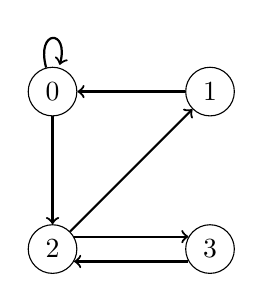
\begin{tikzpicture}
    \node[shape=circle,draw=black] (A) at (0,2) {0};
    \node[shape=circle,draw=black] (B) at (2,2) {1};
    \node[shape=circle,draw=black] (C) at (0,0) {2};
    \node[shape=circle,draw=black] (D) at (2,0) {3};
    \path  (A) edge [loop above, thick] (A);
    \path [->] (B) edge [thick] (A);  
    \path [->] (A) edge [thick] (C);  
    \path [->] (C) edge [thick] (B);  
    \path [->] (C.30) edge [thick] (D.150);  
    \path [->] (D.210) edge [thick] (C.-30);  
    \end{tikzpicture}
    \caption{The defined graph when $b = 4$. There are 4 nodes, each one corresponding to a value mod 4.}
    \label{fig:base_4_graph}
\end{figure}
There are 4 different nodes: one for each integer between 0 and 3. Because $4 = 2^2$, we are looking at the last 2 bits of each number. For example, a number congruent modulo to $0\Mod{4}$ has 00 as the 2 least significant bits, while a number congruent modulo to $2\Mod{4}$ has 10 as its 2 least significant bits. 
\subsection{Base 4 graph construction} \label{subsubsec:proofbase4graph}
Figure~\ref{fig:base_4_graph} shows the Base 4 Collatz Graph, and this subsection describes the construction of it. First, we will start with the even nodes, then the odd nodes:
\begin{itemize}
    \item Node 0 corresponds to the number ending with binary string ``00''. Removing the last 0 leaves either ``00'', looping to $0\Mod{4}$, or ``10'', changing it to $2\Mod{4}$.
    \item Node 2 corresponds to the number ending with binary string ``10''. Removing the last 0 leaves either ``01'', changing it to $1\Mod{4}$, or ``11'', changing it to $3\Mod{4}$.
\end{itemize}
Now, the odd nodes:
\begin{itemize}
    \item Node 1 corresponds to the number ending with binary string ``01''. Multiplying this by 3 and adding 1 results in the binary number ending in ``$y_200$'', where $y_2$ is an unknown bit. Even though we don't know $y_2$, the number is still $0\Mod{4}$.
    \item Node 3 corresponds to the number ending with binary string ``11''. Multiplying this by 3 and adding 1 results in the binary number ending in ``$y_3y_210$'', which is still $2\Mod{4}$.
\end{itemize}
\subsection{Base 4 variants} \label{subsubsec:base4variants}
We introduced the Base 4 case for nodes because we can prove that we need to visit all of the nodes in this graph. This is equivalent to saying that each of the Collatz Variants, $\ColMod{N}{A}{4}$ terminates for nonempty $A \subseteq \{0,1,2,3\}$, and for any input number $N$. 
\begin{theorem}
Algorithm 4 terminates for nonempty $A \subseteq \{0,1,2,3\}$.
\end{theorem}
\begin{proof}
We will start with proving that $\ColMod{N}{2}{4}$ will terminate for any input number $N$, because the 2 node is central to the Base 4 graph.\par
\begin{lemma}
\label{lem:collatzSubTwoModFour}
$\ColMod{N}{2}{4}$ terminates for any $N$.
\end{lemma} 
\begin{proof}
We use the graph to help in this proof. An equivalent question is this: Can we show that node 2 must be visited for all input numbers? To show that this is the case, we have to show that all other nodes must visit node 2. 
\begin{itemize}
    \item 2: If the input number is this, we are already done.
    \item 3: This must, by definition, transition after the $3x+1$ mapping has been applied in one step.
    \item 1 and 0: 1 must transition to 0 after applying the $3x+1$ mapping once. For 0, use Lemma~\ref{lem:zeroCycle}(the ``0 cycle'' lemma) for $b = 4$, and the number will eventually transition to the 2 node.
\end{itemize}
Since all other nodes must visit node 2, it means that for all $N$, $\ColMod{N}{2}{4}$ terminates.
\end{proof} \par

\begin{lemma}
\label{lem:collatzSubOneModFour}
$\ColMod{N}{1}{4}$ terminates for any $N$.
\end{lemma}
\begin{proof}
We use Lemma~\ref{lem:collatzSubTwoModFour} to show that we need to visit node 2, and Lemma~\ref{lem:oneConsumption} to show that the cycle between nodes 2 and 3 cannot continue indefinitely, so node 2 must eventually transition to 1, proving termination of this variant.
\end{proof}
\begin{lemma}
\label{lem:collatzSubZeroModFour}
$\ColMod{N}{0}{4}$ terminates for any $N$.
\end{lemma}
\begin{proof}
Given Lemma~\ref{lem:collatzSubOneModFour}, we know we must visit node 1, and given Lemma~\ref{lem:numOutEdges}, an odd node can only have one outgoing edge, so it must transition to node 0.
\end{proof}
\begin{lemma}
\label{lem:collatzSubThreeModFour}
$\ColMod{N}{3}{4}$ terminates for any $N$.
\end{lemma}
\begin{proof}
Given Lemma~\ref{lem:EvenDom}, the $2 \rightarrow 1 \rightarrow 0 \rightarrow 2$ cycle cannot continue forever because if we assume that the 0 node never self-cycles, $2^2 > 3^1$. The 0 self-cycle makes even nodes dominate in number. So either $\ColMod{N}{3}{4}$ terminates by eventually becoming 1, or the cycle is broken... the only other node to visit is 3, also causing $\ColMod{N}{3}{4}$ to terminate.
\end{proof}
Since all of these lemmas hold, it follows that any singleton set from $A \subseteq \{0,1,2,3\}$ causes $\ColMod{N}{A}{4}$ to terminate. Also, by definition of Algorithm~\ref{alg:ColSP}, any larger size sets for $A$ also terminate as larger set sizes add more termination conditions.
\end{proof}
\section{Base 8 Graph and Variants} \label{subsec:base8graphsubpblms}
We showed that, using the Base 4 graph, $\ColMod{N}{A}{4}$ terminates for any nonempty base set $A$ and input number $N$. We decided to see what would happen if we expanded to $k = 3$ bits. We ran into a problem, and could not prove all variants of $\ColMod{N}{A}{8}$. This will motivate further computation undertaken in chapter~\ref{sec:subhrdnspred}, as we try to determine how hard figuring out these variants are. \par
Figure~\ref{fig:base_8_graph} shows the base 8 graph.
\begin{figure}
    \centering
    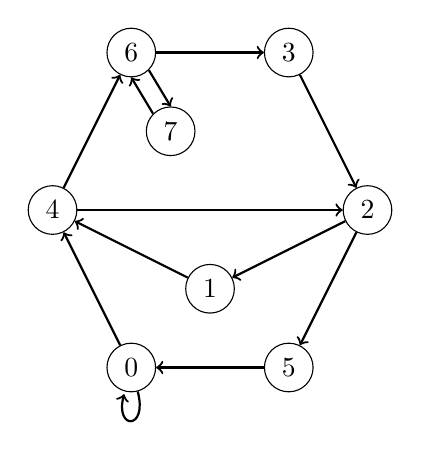
\begin{tikzpicture}
    \node[shape=circle,draw=black] (A) at (1,0) {0};
    \node[shape=circle,draw=black] (B) at (2,1) {1};
    \node[shape=circle,draw=black] (C) at (4,2) {2};
    \node[shape=circle,draw=black] (D) at (3,4) {3};
    \node[shape=circle,draw=black] (E) at (0,2) {4};
    \node[shape=circle,draw=black] (F) at (3,0) {5};
    \node[shape=circle,draw=black] (G) at (1,4) {6};
    \node[shape=circle,draw=black] (H) at (1.5,3) {7};
    \path  (A) edge [loop below, thick] (A);
    \path [->] (A) edge [thick] (E);  
    \path [->] (B) edge [thick] (E);  
    \path [->] (C) edge [thick] (B);  
    \path [->] (C) edge [thick] (F);  
    \path [->] (D) edge [thick] (C);  
    \path [->] (E) edge [thick] (C);  
    \path [->] (E) edge [thick] (G);  
    \path [->] (F) edge [thick] (A);  
    \path [->] (G) edge [thick] (D);  
    \path [->] (G.-45) edge [thick] (H.90);  
    \path [->] (H.135) edge [thick] (G.-90);  
    \end{tikzpicture}
    \caption{The defined graph when $b = 8$. There are 8 nodes, each one corresponding to a value mod 8.}
    \label{fig:base_8_graph}
\end{figure}
There are 8 different nodes, since $8 = 2^3$, and we are looking at the last 3 bits of each number. 
\subsection{Base 8 graph construction} \label{subsubsec:base8proof}
Like the base 4 graph, let us show how to construct the base 8 graph. Like in the base 4 case, let us examine the even nodes first. In this case, there are four different nodes: 0, 2, 4, and 6. Using Lemma~\ref{lem:numOutEdges}, each vertex has two different transitions, depending on what the next bit to the left of the 3 bits after removing the least significant 0. 
\begin{itemize}
    \item Node 0 corresponds to the binary string ``000''. Removing the last 0 leaves either ``000'', looping to $0\Mod{8}$, or ``100'', changing it to $4\Mod{8}$.
    \item Node 2 corresponds to the binary string ``010''. Removing the last 0 leaves either ``001'', changing it to $1\Mod{8}$, or ``101'', changing it to $5\Mod{8}$.
    \item Node 4 corresponds to the binary string ``100''. Removing the last 0 leaves either ``010'', changing it to $2\Mod{8}$, or ``110'', changing it to $6\Mod{8}$.
    \item Node 6 corresponds to the binary string ``110''. Removing the last 0 leaves either ``011'', changing it to $3\Mod{8}$, or ``111'', changing it to $7\Mod{8}$.
\end{itemize}
Now, the odd nodes. Let $y_3$ and $y_4$ be unknown bits.
\begin{itemize}
    \item Node 1 corresponds to the binary string ``001''. Multiplying this by 3 and adding 1 results in the string ``100'', or $4\Mod{8}$.
    \item Node 3 corresponds to the binary string ``011''. Multiplying this by 3 and adding 1 results in the string ``$y_3010$'', which is $2\Mod{8}$.
    \item Node 5 corresponds to the binary string ``101''. Multiplying this by 3 and adding 1 results in the string ``$y_4y_3000$'', which is $0\Mod{8}$.
    \item Node 7 corresponds to the binary string ``111''. Multiplying this by 3 and adding 1 results in the string ``$y_4y_3110$'', which is $6\Mod{8}$.
\end{itemize}
\subsection{Cycle analysis} \label{subsubsec:cycleanalysis}
Since we do not have proofs for all Collatz Variants of base 8 with singleton $A$, we analyzed whether certain cycles can last indefinitely. Some of these analyses can be used in proving some Collatz Variants, whereas others that are unknown can be tied to variants we have not proven yet.
\begin{itemize}
    \item The 0 self-cycle, ($0  \rightarrow \ldots$) cannot continue forever, as per Lemma~\ref{lem:zeroCycle}.
    \item The $6 \rightarrow 7 \rightarrow 6$ cycle cannot continue forever as per Lemma~\ref{lem:oneConsumption}.
    \item The $4 \rightarrow 2 \rightarrow 1 \rightarrow 4$ cycle cannot continue forever, as even nodes dominate ($2^2 > 3$), so according to Lemma~\ref{lem:EvenDom}, this cycle cannot last forever.
    \item $4 \rightarrow 2 \rightarrow 5 \rightarrow 0  \rightarrow \ldots \rightarrow 4$ cycle:  Even nodes dominate, even without any 0 self-cycles ($2^3 > 3$, so according to Lemma~\ref{lem:EvenDom}, this cycle cannot continue forever.
    \item $4 \rightarrow 6 \rightarrow 3 \rightarrow 2 \rightarrow 1 \rightarrow 4$ cycle: There are three different variations of this cycle. We have a proof for only one of them:
\begin{itemize}
  \item No transition allowed from $4 \rightarrow 2$: The following theorem explains this case.
  \begin{theorem} Aaronson '17: The $4 \rightarrow 6 \rightarrow 3 \rightarrow 2 \rightarrow 1 \rightarrow 4$ cycle cannot continue indefinitely.
  \end{theorem}
  \begin{proof}
    If we start some number $x$ such that $x \equiv 4\Mod{8}$, and follow the $4 \rightarrow 6 \rightarrow 3 \rightarrow 2 \rightarrow 1 \rightarrow 4$ cycle once, we turn $x$ into $(9x+20)/8 = \frac{9}{8}(x+20)-20$. If we were to repeat the cycle $k$ times, we would turn $x$ into $\frac{9}{8}^k(x+20)-20$. This quantity must be an integer for all $k$ if the cycle is to continue forever. However, $x+20$ will only have a finite number of factors of 8, so the cycle must terminate.
  \end{proof}
  \item Transition allowed between $4 \rightarrow 2$: This creates a conflict between two different cycles: one that causes growth by approximately a factor of $9/8$ ($4 \rightarrow 6 \rightarrow 3 \rightarrow 2 \rightarrow 1$), and another that causes the cycle to decay by $4/3$ ($4 \rightarrow 2 \rightarrow 1$). This combintation of cycles is one of the more challenging cases to show that we cannot continue indefinitely and no proof is known that we must visit either node 5 or 7. Naturally, a proof would prove termination of variant $\ColMod{N}{\{5,7\}}{8}$, which we explore in section~\ref{sec:subhrdnspred}.
  \item We can also consider visits to the node 7 as well in this cycle. Since each iteration of the $6 \rightarrow 7 \rightarrow 6$ adds one even node and one odd node, $3^{|N_o|} > 2^{|N_e|}$ as before. This proof is arguably harder than the prior proof. A proof of this cycle would solve $\ColMod{N}{\{5\}}{8}$.
\end{itemize}
\item $4 \rightarrow 6 \rightarrow 3 \rightarrow 2 \rightarrow 5 \rightarrow 0 \rightarrow \ldots \rightarrow 4$ cycle: There are three different variations to showing this cycle cannot continue forever, all of them unproven, and all of them lead to interesting questions.
    \begin{itemize}
        \item Strictly following this cycle, no changes: assuming no zero-cycles, there are 4 distinct even nodes in this cycle, and 2 distinct odd nodes $2^4 > 3^2$, so according to the ``Even Node Dominiance Lemma'',~\ref{lem:EvenDom}, this cycle cannot continue forever. The nodes that must be visited to break this cycle are either 1 or 7, so this is a proof that $\ColMod{N}{\{1,7\}}{8}$ terminates.
        \item Allowing 7 but avoiding 1: Like the variant $\ColMod{N}{\{5,7\}}{8}$, we have two conflicting cycles: the $6 \rightarrow 7 \rightarrow 6$ cycle which cause the number to grow by 3/2 every time it takes this cycle, and the base cycle $4 \rightarrow 6 \rightarrow 3 \rightarrow 2 \rightarrow 5 \rightarrow 0 \rightarrow \ldots \rightarrow 4$ that reduces it by at least an approxmiate factor of $\frac{16}{9}$, depending on number of zero self cycles. A proof that the combination of these cycles cannot continue forever would be equivalent to proving terminaton of $\ColMod{N}{\{1\}}{8}$. We present analysis of hardness of this cycle in chapter~\ref{sec:subhrdnspred}.
        \item Allowing 1 but avoiding 7: Adding back in 1 actually allows for three different cycles: $4 \rightarrow 6 \rightarrow 3 \rightarrow 2 \rightarrow 5 \rightarrow 0 \rightarrow \ldots \rightarrow 4$, $4 \rightarrow 6 \rightarrow 3 \rightarrow 2 \rightarrow 1$, and $4 \rightarrow 2 \rightarrow 1$. Naturally, if we can't prove that the simpler combination of cycles $4 \rightarrow 6 \rightarrow 3 \rightarrow 2 \rightarrow 1$, and $4 \rightarrow 2 \rightarrow 1$ cannot terminate, it would be far more difficult to add a third cycle. Solving that the combination of these three cycles must terminate is equivalent to proving termination of $\ColMod{N}{7}{8}$.
    \end{itemize}
\end{itemize}
\subsection{Base 8 variants} \label{subsubsec:base8subprob}
As for which nodes we are forced to visit during the computation of a $3x+1$ sequence, we can prove these four following Collatz Variants terminate:
\begin{itemize}
\item $\ColMod{N}{\{2\}}{8}$
\item $\ColMod{N}{\{3\}}{8}$
\item $\ColMod{N}{\{4\}}{8}$
\item $\ColMod{N}{\{6\}}{8}$
\end{itemize}
$\ColMod{N}{\{0\}}{8}$ can also be shown to terminate but it is entirely dependent on proving another unproven variant. It will still be mentioned here. The following will explain how these five variants terminate.
\begin{itemize}
    \item \textbf{$\ColMod{N}{\{6\}}{8}$}: In the graph, not visiting node $6$, means the Collatz Sequence would have to traverse one of two cycles: $4 \rightarrow 2 \rightarrow 1$ or $4 \rightarrow 2 \rightarrow 5 \rightarrow 0 \rightarrow \ldots \rightarrow 4$, both of which were mentioned in the cycle anaysis as terminating. So $\ColMod{N}{\{6\}}{8}$ must terminate.
    \item \textbf{$\ColMod{N}{\{3\}}{8}$}: We know that $\ColMod{N}{\{6\}}{8}$ terminates, so as a result, we know that node 6 must be visited in our base 8 graph.  Given Lemma~\ref{lem:oneConsumption}, the $6 \rightarrow 7 \rightarrow 6$ cycle cannot continue forever. Hence, $6\Mod{8}$ must transition to $3\Mod{8}$ eventually, meaning $\ColMod{N}{\{3\}}{8}$ terminates.
    \item \textbf{$\ColMod{N}{\{2\}}{8}$}: Since we know that we must visit node 3, this transitions to node 2, proving $\ColMod{N}{\{2\}}{8}$ must terminate.
    \item \textbf{$\ColMod{N}{\{4\}}{8}$}: Given that we know we need to visit node 2, we look at the graph and see two possible paths, both which lead to node 4: Either visit node 1 then 4, or visit node 5 then 0. From Lemma~\ref{lem:zeroCycle}, the 0 cycle cannot continue forever, so the number will eventually transiiton to node 4. Hence, $\ColMod{N}{\{4\}}{8}$ terminates.
    \item \textbf{$\ColMod{N}{\{0\}}{8}$}: In the graph, we can see that to visit node 0, we must come from node 5. So we cannot prove this yet unless we prove termination for $\ColMod{N}{\{5\}}{8}$.
\end{itemize}
We do not have proofs for \item $\ColMod{N}{\{1\}}{8}$, \item $\ColMod{N}{\{5\}}{8}$, \item $\ColMod{N}{\{7\}}{8}$, or the combination of \item $\ColMod{N}{\{5,7\}}{8}$, all of which were mentioned in the cycle analysis. Hence, we've run some computational experiments to try and better understand the difficulty of coming up with a proof for termination of these variants. 


\chapter{Variant Hardness Prediction} \label{sec:subhrdnspred}
In this section, we attempt to determine how difficult variants from Algorithm~\ref{alg:ColSP} are for $\ColMod{N}{A}{8}$, where $A= \{1\}$, $\{5\}$, $\{7\}$, or $\{5,7\}$. We start by defining some measures, talk about the process how we ran experiments, and talk about the results, analyzing termination of the singleton set $A$ Collatz Variants 1, 5, and 7, and the combined 2-element variant of $\{5,7\}$ in separate sections. 
\section{Defining Measures} \label{subsec:algdefinemeasure} 
We define hardness off of the notion that odd numbers make the Collatz Conjecture harder, whereas even numbers make it easier. To more precisely define the measures, define the following numbers, given some input number $x$:
\begin{itemize}
    %\item $x_i$: the number $x$ turns into after $i$ steps of the Collatz Mapping have been applied.
    \item $f(x)$: The total number of steps in the sequence for $x$ before it converges to 1.
    \item $f_\text{odd}(x)$: Number of odd numbers visited in the sequence from $x$ to 1.\footnote{If one wanted to figure out the number of visited even numbers, then $f_\text{even}(x) = f(x) - f_\text{odd}(x)$} 
    \item $A$: The base avoidance set. Same as defined in Algorithm~\ref{alg:ColSP}. For the Collatz Variants we are exploring in this chapter, $A \subseteq \{1, 3, 5, 7\}$ and $A \ne \varnothing$.
    \item $g(x,A)$: The highest number of steps, for an input number $x$ that converges to 1, where $\forall a \in A$, $x_i \not\equiv a \Mod{8} \wedge x_i > 1$. This is counting the maximum number of steps before $\ColMod{N}{A}{8}$ would terminate for input number $N$.
    \item $g_\text{odd}(x,A):$ The number of odd numbers within the given $g(x,A)$
    \item Slice: a batch of numbers from some low number to some high number for a fixed $A$.
    \item $x_{\min}$: the lowest number of any slice.
    \item $x_{\max}$: the highest number of any slice.

    \item Record: any number $r$ in the range that has $g(r,A)$ higher than all numbers measured so far in the slice. More formally, any new record $r_\text{new}$ must have the properties compared to the current record $r_\text{current}$: $r_\text{new} > r_\text{current}$, and $g(r_\text{new},A) > g(r_\text{current},A)$ for a specific $A$. Note that we measure records off of total steps, \textit{not} total number of odd numbers.
      
\end{itemize}
Using these numbers, two different measures are defined, and the intuition behind why they were chosen is given as well: \par
\textbf{Hardness}: Defined to be $H(x,A) = \frac{g_\text{odd}(x,A)}{\log_2{x}}$. This assesses whether or not increasing the number of bits needed to represent the number $x$ changes the difficulty of determining a proof for Collatz Variants  1, 5, or 7, or $\{5,7\}$.  \par
Also define ``Classical Hardness'' as a comparison: $H_C(x) = \frac{f_\text{odd}(x)}{\log_2{x}}$. This computes $H$ with respect to the whole sequence, instead of trying to avoid specific numbers. Records for Classical Hardness occur when $r_\text{new} > r_\text{current}$ and $f(r_\text{new}) > f(r_\text{current})$. \par
\textbf{Percentage of Sequence}: Defined to be $P(x,A) = \frac{g_\text{odd}(x,A)}{f_\text{odd}(x)}$. This assesses what percentage of all odd numbers lie within the longest sequence for Collatz Variants 1, 5, 7, or $\{5,7\}$.

\section{Generating Results} \label{subsec:algcomp}
We wrote a program that computed Collatz Sequences using Java, and ran it on all odd numbers from 1 to 1 billion. The program has various modes which evolved over the lifetime of this project. In these modes, let $\mathcal{A}$ be a family of avoidance sets $A$ we wish to compute.
\begin{itemize}
    \item {\tt baseavoid} is the default option. This allows us to check all $A \in \mathcal{A}$ by running through all odd numbers from $x_{\min}$ (we usually use 1) to $x_{\max}$ (we usually use 1 billion), and determines the maximum number of steps we can run Algorithm~\ref{alg:ColSP} for each set $A \in \mathcal{A}$, or in other words, compute $g(x,A)$ for all odd $x$ in the range $x_{\min} \leq x \leq x_{\max}$. When it finishes, it prints out the longest sequence for each $A$.
    \item {\tt entirechain} just runs Algorithm~\ref{alg:ColR} for all odd $x$ in the range $x_{\min} \leq x \leq x_{\max}$, and prints out the longest sequence.
    \item {\tt untildecay} means that, for each odd number in between $x_{\min}$ and $x_{\max}$, we continue to run until we have a number lower than the original number. We return only the longest sequence of numbers that occurs until the resulting number is smaller than the initial number.
    \item {\tt updown} is a quite different mode. For each odd number $x$ such that $x_{\min}\leq x \leq x_{\max}$, determine two things. First, the number of steps it takes for $x$ to become some number $x_i$ such that $x_i < x$. Second, the number of steps it takes for another number $x_g$ to grow to $x$ if such an $x_g$ exists (no multiple of 3 can grow from a smaller number, for instance). The output prints out, for all odd numbers in the range, $x_i$, the number of steps it takes for $x$ to turn into $x_i$, and, if $x_g$ exists, the number $x_g$ and the number of steps it takes for $x_g$ to grow into $x$.
    \item {\tt avoidingmodgrowth} is a mode like baseavoid. However, it prints tables showing progressively growing records. This is the mode we used to generate the hardness results in this Thesis.
\end{itemize}
As mentioned, we used the {\tt avoidingmodgrowth} mode to generate the records defined in subsection~\ref{subsec:algcomp}. We run for sequences of odd numbers in multiple slices, usually 8, in order to take advantage of parallel computing via a distributed computing program called Condor that was made by The University of Wisconsin-Madison~\cite{Thain:2005:DCP:1064323.1064336}. We then combine the records of these 8 tables by hand using the defined record criterion. \par
We run sequences of numbers and have an option to avoid recomputing odd numbers already part of a prior Collatz Sequence, as these will never generate new records. However, this option can be disabled if we wish to compute extremely large numbers and slices, and are limited in our memory storage. \par
The program could have been rewritten to build off of previously used results, which should run faster, but this would have been difficult without many GBs of memory available and tight memory management on our program. So the space efficient approach was chosen for this project.
\section{Single Base Avoidance Analysis} \label{subsec:algsinglebase}
Our analysis for analyzing the termination of Collatz Variants 1, 5, and 7 is broken into three subsections: two exploring our defined computations, $H$ and $P$, and a third one analyzing interesting properties of sequence similarities that may provide insight to eventual proofs showing that these three Collatz Variants must terminate.
For exploring $H$ and $P$, we took all of the records for Collatz Variants 1, 5, and 7, and plotted the log of all records $r$ versus $H(x,A)$ and $P(x,A)$, respectively. We also added in Collatz Variant 3 as a reference for both of these measures as a control case.
\subsection{Hardness Function Results and Analysis} \label{subsubsec:algsinhardness}
Figure~\ref{fig:hvslog} shows the results of $H(x,A)$ versus the number of bits ($\log_2{x}$). Total steps for each mod number were also added in as well.\par
\begin{figure}
    \centering
    \includegraphics[scale=0.6]{ModAvoidanceAnalysisPics/H_vs_log.png}
    \caption{This graph visualizes how the $H$ values for Collatz Variants 1, 3, 5, and 7 compare to each other, and to classical hardness. The log of the record holding numbers, or number of bits needed, is the x-axis, and the hardness measure $H$ as defined in subsection~\ref{subsec:algdefinemeasure} is the y-axis.}
    \label{fig:hvslog}
\end{figure}
Comparing the three unproven Collatz Variants 1, 5, and 7 to the proven variant 3, the known variant is easier. The known variant actually slight decreases in hardness as the number of bits increases, meaning that there are fewer odd numbers per bit than the unproven variants. \par
Comparing the unknown variants to themselves, there is no consistent leader among the three as the number of bits increases. However, they all seem to be around within a hardness range of 1-3, with only a couple of exceptions. Variant 7 seems to remain in the same range with no definite increase or decrease, whereas variants 1 and 5 grow slightly from around 12 bits onward. The growth for both variants 1 and 5 may be because as numbers get larger, there are more opportunities to visit the $6 \rightarrow 7 \rightarrow 6$ cycle, which clearly adds odd numbers more quickly to the sequence than any other base 8 graph traversal. More experiments for higher numbers should be consider in order to determine whether any of these three unknown variants trend the same way as we add more bits into the computation.\par
Classical Hardness actually tends to grow linearly against the log scale, meaning that as the input number increases, the hardness increases logarithmically. This contrasts to all three unproven variants, which tend to stay between values of 1.5 and 3 for $H$ for numbers below 1 billion, meaning that figuring out proofs for the variants' termination is expected to be easier than proving the Collatz Conjecture.
\subsection{Percentage of Sequence Function Results and Analysis} \label{subsubsec:algsinpercentage}
 Figure~\ref{fig:pvslog} shows the results of $P(x,A)$ versus the number of bits. $P(x,A)$, as discussed earlier, is just calculating what percentage of the record sequence contributes to the overall decay of that sequence to 1. \par
\begin{figure}
    \centering
    \includegraphics[scale=0.6]{ModAvoidanceAnalysisPics/P_vs_log.png}
    \caption{This graph visualizes how the $P$ values for Collatz Variants 1, 5, and 7 compare to each other. The log of the record holding numbers, or number of bits needed, is the x-axis, and the percentage measure $P$ as defined in subsection~\ref{subsec:algdefinemeasure} is the y-axis.}
    \label{fig:pvslog}
\end{figure}
Collatz Variant 7 comprises the highest percentage overall, with a couple of exceptions. Following Collatz Variant 7 causes the sequence to decline rapidly, since the $6 \rightarrow 7 \rightarrow 6$ cycle causes an input number to grow faster than any other cycle in the base 8 graph. Almost all of the records for variant 7 terminate at 1 instead of actually reaching a number that is $7 \Mod{8}$. \par
Variant 5 tends to have a low percentage, and appears to be the least erratic of all four variants. Variant 5 avoids the 0 self-cycle, which causes many divisions by 2. Numbers having a long sequence that prevent termination of variant 5 tend to have a very large number when they finally reach a number that is $5 \Mod{8}$, meaning that often, many more steps in the $3x+1$ mapping must be taken before these numbers converge to 1. \par
Variant 1 is interesting, because as the input numbers grow larger, the line changes from erratic behavior to a more steady percentage between approximately 50\% and 60\% at around 20 bits. This is likely a consequence of the sequence similarity that is seen in larger record for variant 1, which will be analyzed in subsubsection~\ref{subsubsec:algseqsim}. Further, as mentioned in the cycle analysis in subsection~\ref{subsubsec:cycleanalysis}, the $4 \rightarrow 6 \rightarrow 3 \rightarrow 2 \rightarrow 5 \rightarrow 0 \rightarrow \ldots \rightarrow 4$ cycle combined with the  $6 \rightarrow 7 \rightarrow 6$ cycle which avoidings node 1 causes a clash between the decay of the 0 self-cycle and the growth of the $6 \rightarrow 7 \rightarrow 6$ cycle, which may explain some of the erratic behavior for variant 1, aside from the small part with chain similarity. \par
Variant 3 tends toward the lowest percentage of all odd numbers, even lower than variant 5, but also has erratic behavior. This could be explained by the fact that avoiding termination of variant 3 causes the sequence to follow some combination of the $6 \rightarrow 7 \rightarrow 6$ cycle, the $4 \rightarrow 2 \rightarrow 1 \rightarrow 4$ cycle, or the $4 \rightarrow 2 \rightarrow 5 \rightarrow 0  \rightarrow \ldots \rightarrow 4$ cycle with some number of $0$ self-cycles. The first cycle causes growth, whereas all three other cycles cause decay. If the growth cycle is followed, the number gets larger, likely reducing the percentage of odd numbers making up long chains avoiding termination of variant 3, whereas the decay cycles cause the number to shrink, tending the percentages to be higher. This may explain why variant 3 causes widely different percentages.
\subsection{Sequence similarity analysis} \label{subsubsec:algseqsim}
We analyzed the sequences of the records for Collatz Variants 1, 5, and 7 as well to see if we could find any similarities:
\begin{itemize}
    \item Variant 1: There are two groups of records that were particularly interesting: Those from 325,791 to 32,505,681 (call this group $S$), and those from 35,651,835 to 949,643,331 (call this group $T$). Group $S$ numbers all terminated at number 161, and group $T$ numbers all terminated at number 35,369. These sequences all matched \textit{number-by-number} at least one other sequence starting at most 8 steps from the beginning. This is a striking similarity meaning that records for variant 1 might be predictably related to groups $S$ or $T$, or perhaps to other groups.
    \item Variant 7: All record sequences, except for input number 27, terminated at 1. While there was some similarity between sequences (all numbers $\geq 62079$ had the same last 41 numbers), there were many different paths taken from the input, so not as many patterns here.
    \item Variant 5: This had few matches and was the most changing of the records, so chain similarity appears not to have did not have as much to do with the low variance that $P$ has for variant 5.
\end{itemize}
\section{Paired Base Avoidance Analysis} \label{subsec:algpairedbase}
Since termination of Collatz Variants 1, 5, and 7 appear to be difficult to prove, we also analyzed two element combinations of them. The termination of two such variants were already proved in subsection~\ref{subsubsec:base8subprob}: $\{1,5\}$ and $\{1,7\}$. However, termination of variant $\{5,7\}$ is unknown. This section will analyze what happens to $H(x,A)$ and $P(x,A)$ where $A=\{1,5\}$, $\{1,7\}$, and $\{5,7\}$.
\subsection{Hardness Function Results and Analysis} \label{subsubsec:algmulhardness}
\begin{figure}
    \centering
    \includegraphics[scale=0.6]{ModAvoidanceAnalysisPics/H_vs_log_multi_base.png}
    \caption{This graph visualizes the $H$ measure for the three Collatz Variants $\{1,5\}$, $\{1,7\}$, and $\{5,7\}$. The log of the record holding numbers, or number of bits needed, is the x-axis, and the hardness measure $H$ as defined in subsection~\ref{subsec:algdefinemeasure} is the y-axis. Classical Hardness was omitted from this graph to eliminate distortion.}
    \label{fig:h_multivslog}
\end{figure}
Figure~\ref{fig:h_multivslog} shows the results of $H(x,A)$ versus $\log_2{x}$. These results were quite surprising. At first thought, it would have appeared that the unproven variant $\{5, 7\}$ should be the hardest to determine, compared to the two variants we have proofs for. But both variants $\{1, 5\}$ and $\{1, 7\}$  had alike predictive hardness to $\{5, 7\}$! These numbers suggest that a proof for determining why variant $\{5, 7\}$ must terminate is either easier than we anticipated, or our hardness measures are not very good. However, given the fact that variant 3 for the single base cases is clearly easier than variants 1, 5, and 7, we have reason to believe this measure should be good. Further investigation needs to be considered.
\subsection{Percentage of Sequence Function Results and Analysis} \label{subsubsec:algmulpercentage}
\begin{figure}
    \centering
    \includegraphics[scale=0.6]{ModAvoidanceAnalysisPics/P_vs_log_multi_base.png}
    \caption{This graph visualizes the $P$ measure for variants $\{1,5\}$, $\{1,7\}$, and $\{5,7\}$. The log of the record holding numbers, or number of bits needed, is the x-axis, and the hardness measure $P$ as defined in subsection~\ref{subsec:algdefinemeasure} is the y-axis.}
    \label{fig:p_multi_vslog}
\end{figure}
Figure~\ref{fig:p_multi_vslog} shows the results of $P(x,A)$ versus $\log_2{x}$. The variant $\{1,7\}$ makes up the highest percentage of the sequence compared to the other two cases, because avoiding both the $6 \rightarrow 7 \rightarrow 6$ and the $4 \rightarrow 6 \rightarrow 3 \rightarrow 2 \rightarrow 1 \rightarrow 4$ cycles only allows for the sequence to go through the $4  \rightarrow 2 \rightarrow 5 \rightarrow 0 \rightarrow \ldots \rightarrow 4$ cycle, causing fast decay, like with variant 7. \par
Both variants $\{1,5\}$ and $\{5,7\}$ are much closer to each other in percentage of total sequence, although as the numbers grow past 17 bits in size, variant $\{5,7\}$ comprises of the higher percentage of the sequence. A possible explanation is the fact that the $6 \rightarrow 7 \rightarrow 6$ cycle allowed in variant $\{1,5\}$ allows causes a number to grow larger than the $4 \rightarrow 6 \rightarrow 3 \rightarrow 2 \rightarrow 1$ cycle that variant $\{5,7\}$ allows. Also, since variant $\{1,5\}$ allows for larger numbers, and larger numbers generally (but not always) take more steps to decline, allowing for more growth should mean that the long sequence avoiding termination of variant $\{1,5\}$ comprises a lower percentage of all odd numbers.


%MENTION SAT SOLVERS VERY BRIEFLY HERE.

\chapter{String Rewriting Systems (SRS) and SAT Solvers} \label{sec:SRSandSAT}
A string rewriting system (SRS), at a high level, takes a input string of an alphabet, and applies string rewriting rules (SRRs) in an arbitrary order on the input string to see if the string can be transformed further. An example SRS is given.
\begin{definition}{SRS A:} 
The alphabet is $\Sigma = \{a, b, c\}$ and the SRRs are as follows:
\begin{enumerate}
    \item $aa \rightarrow bc$
    \item $bb \rightarrow ac$
    \item $cc \rightarrow ab$
\end{enumerate}
\end{definition}
A problem, called Zantema's Other Problem~\cite{Hofbauer:2006:TA:1142725.1711178}, using SRS A, asks the following question:\par\noindent
\begin{question}{Zantema's Other Problem:}
Does the system laid out in SRS $A$ terminate for any input string $(a|b|c)*$?
\end{question}
If one thinks about this problem a little, it would seem that a proof to show that this problem terminates for all input strings should be easy to show. \marginnote{I'm unsure of whether I should go into more detail for this section.} Surprisingly, both humans and computers struggled to come up with a proof for this problem when initially presented.  However, Hofbuaer and Waldmann came up with a proof for determining that it terminates~\cite{Hofbauer:2006:TA:1142725.1711178}, and from this, found that, for any rewriting rules in any rewrite system, if they are transformed into functions that causes all inputs to decrease, then the rewrite system will terminate.~\cite{Hofbauer2006}. \par
The matrices are built using SAT solving to determine if a $d \times d$ matrix is large enough to ensure that the matrix functions for the set of rewrite rules always decrease for all inputs. The process of building these matrices is described in a paper by Endrullis, Waldmann and Zantema~\cite{Endrullis2006}. An example using Zantema's Other Problem will be explained here.\par
Here are the matrices computed by SAT from ~\cite{Hofbauer:2006:TA:1142725.1711178}:
%FIX THIS OVERFULL PROBLEM HERE AND IN THE NEXT SET.
\[
a(\Vec{x}) = \begin{pmatrix}
1&0&0&3\\
0&0&2&1\\
0&1&0&1\\
0&0&0&0
\end{pmatrix} \Vec{x} + \begin{pmatrix}
1\\
0\\
1\\
0
\end{pmatrix}
b(\Vec{x}) = \begin{pmatrix}
1&2&0&0\\
0&2&0&1\\
0&1&0&0\\
0&0&0&0
\end{pmatrix} \Vec{x} + \begin{pmatrix}
1\\
2\\
0\\
0
\end{pmatrix}
c(\Vec{x}) = \begin{pmatrix}
1&0&0&1\\
0&0&0&1\\
0&1&0&1\\
0&2&0&0
\end{pmatrix} \Vec{x} + \begin{pmatrix}
1\\
0\\
3\\
0
\end{pmatrix}
\]
We will show an example string to show that it is always decreasing, but first, we need to define an appropriate operator. Define the $\succ$ operator to show that, for vectors $(x_1 \ldots x_d)$ and $(y_1 \ldots y_d)$, $(x_1 \ldots x_d) \succ (y_1 \ldots y_d)$ if $x_1 > y_1$ and $x_i \geq y_i$ for $i \in \{2, \ldots, d\}$. In other words, the first element of a vector must be always decreasing, while the other $d-1$ elements must either be the same or decrease. \par
Let our sample string be $bbaa$. Here is a possible set of rules that can be applied to it as well as the vector representations of the symbols:
%FIX THIS OVERFULL PROBLEM HERE
\begin{align*}
    bb\underline{aa} &\rightarrow b\underline{bb}c &\rightarrow ba\underline{cc} &\rightarrow b\underline{aa}b &\rightarrow \underline{bb}cb &\rightarrow a\underline{cc}b &\rightarrow aa\underline{bb} &\rightarrow a\underline{aa}c &\rightarrow ab\underline{cc} &\rightarrow abab \\
    \begin{pmatrix}18\\14\\6\\0\end{pmatrix} &\succ
    \begin{pmatrix}17\\14\\6\\0\end{pmatrix} &\succ
    \begin{pmatrix}15\\14\\6\\0\end{pmatrix} &\succ
    \begin{pmatrix}14\\14\\6\\0\end{pmatrix} &\succ
    \begin{pmatrix}13\\14\\6\\0\end{pmatrix} &\succ
    \begin{pmatrix}7\\14\\5\\0\end{pmatrix} &\succ
    \begin{pmatrix}6\\14\\5\\0\end{pmatrix} &\succ
    \begin{pmatrix}4\\14\\3\\0\end{pmatrix} &\succ
    \begin{pmatrix}3\\0\\3\\0\end{pmatrix} &\succ
    \begin{pmatrix}2\\0\\3\\0\end{pmatrix}
\end{align*}
The vector representation of the strings are always decreasing as defined by the $\succ$ operator. We could apply any string with symbols $a$, $b$, and $c$ and apply rules until termination and the vectors representing the strings would always decrease.

%I need to make sure that I define subproblems clearly here to mean SRSs with rewrite rules. That's going to be a bit later.

\chapter{Hardness of Application of Rewrite Rules} \label{sec:hardnessrewriterules}
\textbf{****NOTE! This chapter is going to be heavily rewritten for the next iteration. Feel free to look at it now if you have time, but it may be drastically different next time.****}\par
%Outline:
%-Scott mentioned that he expects the number of rewrite steps needed is O(log(N)^2), where N is the input number. My findings are consistent with this. I ran the rewrite system for all Delay Records found on Roosendaal's website up to 1 billion: http://www.ericr.nl/wondrous/delrecs.html
%        -I took steps that the rewrite system and divided by O(log(N)^2). The constant never exceeds 15.37. This is well bounded by the highest Gamma constant I found up to 1 billion: 32.89.
%        -Recall that Gamma is defined by:
%            -Steps to reach 1 = Gamma * ln(N) (From Lagrias's Survey)
%            -The max Gamma found by Eric Roosendaal is 36.72 for approximately 7.2*10^21 (source: http://www.ericr.nl/wondrous/comprecs.html)
%-Hardness of 1, 5, and 7 mod 8 from a rewrite perspective: I'll compute H_r(x,A) = # of rewrite steps we avoid A mod 8/log^2(N), and compare 1, 5, and 7 mod 8 to each other.
%        -I should also do the same with the number of rewrite steps for the normal Collatz Delay Records and compare these to 1, 5, and 7 mod 8.
% -Exploring modifications of the rewrite system:
%        -I used a modified rewrite system that Marijn told me about (eliminating the ad -> d rule) on the Delay Records from Roosendaal's website, and found that we decrease rewrite steps between around 7% - 25%. However, the larger the number, the smaller percentage the decrease.
%        -Want to present results and leave as an open suggested topic for further optimizations. I'm open to taking any other suggestions before I finish this Thesis.



Now we have explained the background for Rewrite Systems, as well as the motivation for them, we now build on top of the  algebraic hardness measure computation done in chapter~\ref{sec:subhrdnspred}. First, we discuss a program we created that replays the Collatz SRS for certain numbers, which is used throughout this chapter. Then, we attempt to establish a reasonable upper bound for number of rewrite steps needed. We then use this upper bound to compute reasonable hardness measures for modifications of the Collatz SRS that align with the earlier discussed variants. Finally, we explore another modification to Aaronson's rewrite system which reduces rewrite steps.% First, we do computations with slight modifications to the Collatz SRS, and second, we only compute record sequences from our previous algebraic analysis. In this section, we first introduce a modified version of the SRS, then we define measures, talk about the computation, then present our results.
\section{Computation} \label{subsec:rewritecomp}
The program we wrote simulates the Collatz SRS in Java. It takes two different keys of input: some positive integers (either one number, or a batch of numbers, one per line), and a string file which has one SRR per line in the format ``input output'', which is equivalent to the rule $input \rightarrow output$. The \# character is a comment, meaning if the first character of a rewrite rule is \#, we ignore that line. This is a convenience to comment out a rule to create SRRs that correspond to Collatz subproblems. \par
The program converts an input number into a binary rewrite string with characters $a$, $b$, $c$, and $d$. The rewrite term is stored in a ``sliding'' array, because in Aaronson's SRS, a number can only add string length from the $c$ rules. When we apply rule $D_1$, for instance, the $a$ term gets replaced with a $d$ term, and a pointer denoting the end of the string gets moved to the new $d$ symbol. If we run out of space in the array, we double the size of it, discarding any trailing $d$ terms. \par
As discussed in section~\ref{sec:CollatzSRS}, we don't apply SRRs in arbitrary order. Given a rewrite string completely in binary, we check to see if any $D$ rule can be applied. If not, the program terminates. If we do find a $D$ rule, then apply it, and check if a ternary character is generated by it. If so, we apply the $A$ and $B$ rules to move the ternary character index-by-index until we can apply a $C$ rule, which removes the ternary character. \par
The input is either a single number, or a batch that is a list of interesting numbers. If a batch of numbers is run, an aggregate file can be printed that lists the input number, the final number, and the number of rewrite steps.

\section{Estimated rewrite steps needed} \label{subsec:estrwsteps}
Looking at how the Collatz SRS operates, one can establish a reasonable bound on the number of steps. Starting with a number that is purely in binary symbols $a$ and $b$, plus the placeholder symbols $c$ and $d$, there are two different paths that occur: one where $a$ is the symbol next to the $d$, meaning we divide by 2. So, it only takes one step to divide by 2. On the other hand, when we compute an odd number, we turn the $b$ symbol into a $g$ symbol, and, following the establised order, apply $A$, $B$, and $C$ rules to conver the ternary symbol to binary. This adds $\Theta(m)$ rewrite steps for the odd number. \par
Since odd rules add hardness to the rewrite system, what we can do is compare the number of steps that the rewrite system takes on Classical Hardness records from chapter~\ref{sec:subhrdnspred}, divide the number of steps that odd terms in the Collatz Sequence take by $\log^2{m}$, and compare it to our Classical Hardness measure to see if the rewrite system asymptotically adds $\Theta(m)$ rewrite steps for each odd term. We have done so, and the results are presented in Figure\#. From this graph, it appears that dividing the odd number of rewrite steps by $\log{m}$ creates a reasonably tight bound against Classical Hardness, so given the numbers we measures, adding a factor or $\Theta(m)$ rewrite steps per odd number appears to be correct, so the number of rewrite steps needed for a $m$ bit input number appears to be $O(m^2)$.

%%%%OK. This stuff about Gamma is NOT needed. Why? Because the Classical Hardness ALREADY IS THE QUANTITY I'M LOOKING FOR!!! IT IS LITERALLY ODD NUMBERS DIVIDED BY BITS!
%So what do I need to do? Just take the rewrite system, divide it by $\log{m}$ TWICE, and see how it trends compared to classical hardness!!!!
%Therefore, we need to know what is the number of odd numbers we expect to hit. We can look at Lagrias's surveys to see that he defined some quantity called ``gamma value'', or $\gamma$ for short:
%\[
%\gamma(x) := \frac{\sigma_{\inf}(x)}{\log{x}}
%\] 
%where $\sigma_{\inf}(x)$ is the number of steps it takes for $x$ to reach 1 in $\Col{x}$, except when $x_i$ is odd, the $3x+1$ then immediate division after 2 is counted as one step. Therefore, $\sigma_{\inf}(x) = f_{\text{even}}(x),$ which was defined in section~\ref{subsec:algdefinemeasure}.

\section{Collatz SRS Subproblem Analysis} \label{subsec:collatzsubproblemananalysis}
Although it appears that the rewrite system adds a factor of $\log{m}$ steps to solving the Collatz Conjecture, and that the rewrite system takes $O(m^2)$ steps, this does not mean that the hardness of the Collatz Variants will not differentiate, given the fact that certain variants may deal with different sized numbers. This section takes the Collatz SRS and modifies it to have it effectively compute Algorithm~\ref{alg:SP}
\subsection{Modified Base 8 Rewrite System} \label{subsec:base8rewrite}
Now we have established a reasonable bound of how many more steps the rewrite system adds, let us explore how we can modify the Collatz SRS to make it tie into our variants. Recall the $D$ rules of the Collatz SRS: the rules that handle the even and odd numbers:
\begin{align*}
    D_1: ad &\rightarrow d &\text{$0\Mod{2}$}\\
    D_2: bd &\rightarrow gd &\text{$1\Mod{2}$}\\
\end{align*}
$D_1$ handles $0 \Mod{2}$ (even numbers) by effectively dividing by 2, while $D_2$ handles $1 \Mod{2}$ (odd numbers)  by effectively computing $3x+1/2$. Also note that all input strings for these rules are just one bit, since the placeholder $d$ is not a digit. However, we can expand this input to be 3 bits and come up with 8 corresponding SRRs:
\begin{align*}
    aaad &\rightarrow aad &\text{$0\Mod{8}$}\\
    aabd &\rightarrow ebad &\text{$1\Mod{8}$}\\
    abad &\rightarrow abd &\text{$2\Mod{8}$}\\
    abbd &\rightarrow fabd &\text{$3\Mod{8}$}\\
    baad &\rightarrow bad &\text{$4\Mod{8}$}\\
    babd &\rightarrow gaad &\text{$5\Mod{8}$}\\
    bbad &\rightarrow bbd &\text{$6\Mod{8}$}\\
    bbbd &\rightarrow gbbd &\text{$7\Mod{8}$}
\end{align*}
It is easy to see how these rules all correspond to a node in graph $G_8$: an input string strictly with symbols $a$, $b$, $c$, and $d$ corresponds to a binary number. The inputs, in order, are numbers congruent moduly to 0-7$\Mod{8}$, and the outputs are the result of dividing by 2, if even, or multiplying by 3 and adding 1. All of the odd rules, like rule $D_2$ in the original system, are just a combination of several rules, which ensure that the output string is not longer, and it reduces a couple of steps by moving the ternary term toward the front. All of the even number node rules are just the same exact rule $D_1$ in the original system, so we can remove any even rules and replace them with the original $D_1$. Hence, we use the following SRRs in the base 8 modification of the Collatz SRS:
\begin{align*}
    D_{8_1}: ad &\rightarrow d &\text{$0\Mod{2}$}\\
    D_{8_2}: aabd &\rightarrow ebd &\text{$1\Mod{8}$}\\
    D_{8_3}: abbd &\rightarrow fabd &\text{$3\Mod{8}$}\\
    D_{8_4}: babd &\rightarrow gd &\text{$5\Mod{8}$}\\
    D_{8_5}: bbbd &\rightarrow gbbd &\text{$7\Mod{8}$}
\end{align*}
Because these rules were constructed using only SRRs in the Collatz SRS that we know to be correct, we know these new $D$ rules, plus the $A$, $B$, and $C$ rules, are equal to the original Collatz SRS. However, they do add an extra dimension not present before. We can remove one of the rules to make it easier to prove that the derived SRS will terminate. We present a sample SRS with rule $D_{8_2}$ removed:
\begin{align*}
    D_{8_1}: ad &\rightarrow d &\text{$0\Mod{2}$}\\
    D_{8_3}: abbd &\rightarrow fbbd &\text{$3\Mod{8}$}\\
    D_{8_4}: babd &\rightarrow gd &\text{$5\Mod{8}$}\\
    D_{8_5}: bbbd &\rightarrow gbbd &\text{$7\Mod{8}$}
\end{align*}
Since we removed the SRR that corresponds to input $1 \Mod{8}$, termination of this SRS implies termination of Collatz Variant 1, as removing a rule causes any string with this input to terminate the system. Note how removing an SRR is equivalent to adding the corresponding termination condition in Algorithm~\ref{alg:SP}. Any derived Collatz SRS that alters the base 8 modification of the Collatz SRS will henceforth be referred to as a Collatz Subproblem $A$, where $A$ will bethe same base avoidance set as used in $\ColMod{N}{A}{b}$. For singleton sets $A$, we just write the number. Collatz Subprolem $A$ denotes which rewrite rule(s) are dropped, and that subproblem $A$ would imply termination of Collatz Variant $A$.\par
The rest of this chapter describes the investigation we took to determine the number of steps that Collatz Subproblems 1, 5, and 7 need before terminating.
\subsection{Defining Measures for Subproblem Analysis} \label{subsec:rewritemeasuredefs}
Instead of defining hardness by number of odd numbers, for the SRS, we define hardness based off of the total steps applied, because of the fact that odd numbers add significantly more steps. Define the following numbers, given some input number $x$:
\begin{itemize}
    \item $f_r(x)$: The total number of rewrite steps in the sequence for $x$ before it converges to 1.
    \item $A$: The base avoidance set, same as used in Algorithm~\ref{Col:SP} and chapter~\ref{sec:subhrdnspred}. As before, $A \subseteq \{1, 5, 7\}$ and $A \ne \varnothing$. Dropping an SRR that corresponds to avoiding $a \Mod{8}$  effectively adds $a$ to $A$.
    \item Record Sequence for $A \Mod{b}$: Same exact definition as in chapter~\ref{sec:subhrdnspred}. We only run rewrite systems for the record sequences we computed with the algebraic Collatz method, as running computation for strictly the rewrite system would take an extremely long time.
    \item $R(x, A, b):$ The number of rewrite steps that the record sequence from Collatz Variant $\ColMod{x}{A}{b}$ takes in an SRS based off of Collatz Subproblem $A$. 
\end{itemize}
We define only one hardness measure: $H_{SRS}$, where $H_{SRS} = \frac{R(x, A, b)}{\log_2{x}}$. This effectively computes the hardness of the SRRs that corresponds to determining termination of Collatz Variant $A$.

\subsection{Single SRR removal analysis} \label{subsec:rewritehardness}
Figure~\ref{fig:rvslog} shows the anaylsis of hardness for the modified SRS with removal on one of three different rules. Note that the hardness tends to grow for all three cases, as opposed to the analysis for $H(x,A)$ for each of these three cases, which tend to stay flat. This shows, that as the number of bits increases, the number of steps for the rewrite system tend to increase logarithmically. The best explanation for why this is the case is because for each odd rule, we add $\Theta(\log{n})$ steps, so as discussed in the algebraic case, hardness is determined by odd numbers.
\begin{figure}
    \centering
    \includegraphics[scale=0.75]{ModAvoidanceAnalysisPics/R_vs_log.png}
    \caption{This graph visualizes how the $R$ values for subproblems 1, 5, and 7 compare to each other. The log of the record holding numbers, or number of bits needed, is the x-axis, and the hardness measure $R$ as defined in section~\ref{subsec:rewritemeasuredefs} is the y-axis.}
    \label{fig:rvslog}
\end{figure}
However, it is clear that all three cases don't have the same slope of increase. Subproblem 7 has the most gradual growth of all three cases, followed by subproblem 1 and subproblem 5, which has not only the most growth, but the highest standard deviation of all three cases. These can be explained by the following observations:
\begin{itemize}
    \item Record sequences for subproblem 7 eliminate the growth of the $6 \rightarrow 7 \rightarrow 6$ cycle, meaning the numbers tend to get smaller and need less bits to encode as a rewrite string.
    \item Record sequences for subproblem 5 eliminate the decay of the 0 self-cycle, meaning numbers tend to grow more often than not, so the numbers here are larger.
    \item Record sequences for subproblem 1 is in between the other two cases, since both the 0 self-cycle of decay and the $6 \rightarrow 7 \rightarrow 6$ of growth can occur.
\end{itemize}


\chapter{Conclusion} \label{sec:conclusion}
In this thesis, we analyzed the Collatz Conjecture and simpler, yet still challenging variants, and propose a hardness prediction for determining the answers to these variants. We started by building a program that investigates Collatz Variants by running many $3x+1$ sequences for all odd numbers up to 1 billion, and seeing how many odd numbers occur in record breaking sequences that avoid terminating the Collatz Variants. \par
We also investigated the Collatz SRS that Aaronson created and that Heule tried to prove with matrix interpretation. Even though this methodology has been unable to solve the Collatz Conjecture so far, we think it still has promise. We also built a simple program that ran the Collatz SRS and determined the hardness for subproblems, finding out that the hardness varies more than in the algebraic case.\par
As described in ~\cite{HeuleAaronson}, we believe this approach for trying to solve the Collatz Conjecture, as well as Collatz Variants, has merit and needs further investigation. We plan to do so under the recently approved grant.




%%%%%%%%%%%%%%%%%%%%%%%%%%%%%%%%%%%%%%%%%%%%%%%%%%%%%%%%%%%%%%%%%%%%%%
% Appendix/Appendices                                                %
%%%%%%%%%%%%%%%%%%%%%%%%%%%%%%%%%%%%%%%%%%%%%%%%%%%%%%%%%%%%%%%%%%%%%%
%
% If you have only one appendix, use the command \appendix instead
% of \appendices.
% I MAY have an appendix later on with results.
%\appendices
%\index{Appendices@\emph{Appendices}}%

%\include{Chapters/chapter-appendix1}

%\include{Chapters/chapter-appendix2}

%\include{Chapters/chapter-appendix3}


%%%%%%%%%%%%%%%%%%%%%%%%%%%%%%%%%%%%%%%%%%%%%%%%%%%%%%%%%%%%%%%%%%%%%%
% Generate the bibliography.					     %
%%%%%%%%%%%%%%%%%%%%%%%%%%%%%%%%%%%%%%%%%%%%%%%%%%%%%%%%%%%%%%%%%%%%%%
%								     %
% NOTE: For master's theses and reports, NOTHING is permitted to     %
%	come between the bibliography and the vita. The command      %
%	to generate the index (if used) MUST be moved to before      %
%	this section.						     %
%								     %
\nocite{*}      % This command causes all items in the 		     %
                % bibliographic database to be added to 	     %
                % the bibliography, even if they are not 	     %
                % explicitly cited in the text. 		     %
		%						     %
\bibliographystyle{ieeetr}  % Here the bibliography 		     %
\bibliography{bibliography}        % is inserted.			     %
\index{Bibliography@\emph{Bibliography}}%			     %
%\printbibliography
%%%%%%%%%%%%%%%%%%%%%%%%%%%%%%%%%%%%%%%%%%%%%%%%%%%%%%%%%%%%%%%%%%%%%%


%%%%%%%%%%%%%%%%%%%%%%%%%%%%%%%%%%%%%%%%%%%%%%%%%%%%%%%%%%%%%%%%%%%%%%
% Generate the index.						     %
%%%%%%%%%%%%%%%%%%%%%%%%%%%%%%%%%%%%%%%%%%%%%%%%%%%%%%%%%%%%%%%%%%%%%%
%								     %
% NOTE: For master's theses and reports, NOTHING is permitted to     %
%	come between the bibliography and the vita. This section     %
%	to generate the index (if used) MUST be moved to before      %
%	the bibliography section.				     %
%								     %
%\printindex%    % Include the index here. Comment out this line      %
%		% with a percent sign if you do not want an index.   %
%%%%%%%%%%%%%%%%%%%%%%%%%%%%%%%%%%%%%%%%%%%%%%%%%%%%%%%%%%%%%%%%%%%%%%


%%%%%%%%%%%%%%%%%%%%%%%%%%%%%%%%%%%%%%%%%%%%%%%%%%%%%%%%%%%%%%%%%%%%%%
% Vita page.							     %
%%%%%%%%%%%%%%%%%%%%%%%%%%%%%%%%%%%%%%%%%%%%%%%%%%%%%%%%%%%%%%%%%%%%%%

\begin{vita}
Matthew Alexander Denend was born in Spokane, Washington. He received the Bachelor of Science degree in Electrical Engineering, cum laude, from The University of Washington, Seattle, in 2012. He worked as a Packet Core Performance and Handset Engineer at T-Mobile in Bellevue, Washington for 3 years. He decided to pursue a Master of Science in Computer Science degree, and after he was accepted to The University of Texas at Austin in 2015, he left his job at T-Mobile to move to Austin, Texas and became a full-time student.
\end{vita}

\end{document}
